In this section, we demonstrate the scalability of our proposed cryptosystems.
Our experiments focus on the difficult case when $t > n/2$, specifically $t=f+1$ and $n=2f+1$.
We benchmark TSS, VSS and DKG cryptosystems for thresholds $t \in\{2^1,2^2,2^3,\dots,2^{20}\}$.
Although we did not benchmark other thresholds, similar performance gains would have been observed for other sufficiently large values of $t$ (e.g., $t=f+1$ and $n=3f+1$).
However, we acknowledge that, for sufficiently small $t$, \evss's and \ejfdkg's $\Theta(nt)$ dealing would outperform ours.
Similarly, in this small $t$ setting, naive Lagrange interpolation would outperform fast Lagrange.
Our experiments show that:
\begin{itemize}
    \item Our BLS TSS scales to $n \approx 2$ million signers and outperforms the naive scheme as early as $n=\blsOutperformN$ (see \cref{f:thresh}).
    % Note: Outperforming in the 'worst case'
    \item \ourvss scales to hundreds of thousands of participants, and outperforms \evss as early as $n=\vssOutperformWcN$ (see \cref{f:vss-e2e-times}).
    \item \ourdkg scales to $n\approx$ 65,000 players and outperforms \ejfdkg at $n=\dkgOutperformWcN$ (see \cref{f:dkg-e2e-times}).
\end{itemize}
Importantly, our VSS and DKG speed-ups come at the price of a modest increase in communication (see \cref{f:dkg-bw}).
For example, for $n\approx$ 65,000, a DKG player's communication during dealing increases by \amtDkgCommOverhead{65535} from \ejfDkgComm{65535} in \ejfdkg to \amtDkgComm{65535} in \ourdkg.
However, since the worst-case end-to-end time decreases by \amtDkgEndToEndWcTimeImprovOverejf{65535} from \ejfDkgEndToEndWcTime{65535} in \ejfdkg to \amtDkgEndToEndWcTime{65535} in \ourdkg, the extra communication should be worth it in many applications.

For prohibitively-slow experiments with large $t$, we repeat them fewer times than experiments with smaller $t$.
For brevity, we specify the amount of times we repeat an experiment for each threshold via a \textit{measurement configuration}.
For example, the measurement configuration of our efficient BLS threshold scheme is $\langle 7 \times 100, 13 \times 10 \rangle$.
This means that for the first 7 thresholds $t\in\{2^1,2^2,\dots,2^7\}$ we ran the experiment 100 times while for the last 13 thresholds we ran it 10 times.

\paragraph{Codebase and Experimental Setup.}
We implemented (1) our BLS threshold signature scheme from \cref{s:threshsig}, (2) \ejfdkg~\cite{Kate2010} and \ourdkg and (3) \evss~\cite{KZG10a} and \ourvss in 5700 lines of C++.
We used a 254-bit Barretto-Naehrig curve with a Type~III pairing~\cite{bn-curve} from Zcash's \texttt{libff}~\cite{libff} elliptic curve library.
We used \texttt{libfqfft}~\cite{libfqfft} to multiply polynomials fast using FFT.
All experiments were run on an Intel Core i7 CPU 980X @ 3.33GHz with 12 cores and 20 GB of RAM, running Ubuntu 16.04.6 LTS (64-bit version).
Since all benchmarked schemes would benefit equally from multi-threading, we did not implement it.

\paragraph{Limitations.}
Our DKG and VSS evaluations do not account for network delays.
This is an important limitation.
Our focus was on the computational bottlenecks of these protocols.
Nonetheless, scaling and evaluating the broadcast channel of VSS and DKG protocols is necessary, interesting future work.
In particular, ideas from scalable consensus protocols~\cite{algorand} could be used for this.
Finally, our VSS and DKG ``worst case'' evaluations do not fully account for malicious behavior.
Specifically, they do not account for the additional communication and computational cost associated with complaint broadcasting.
We hope to address this in future work (see \cref{s:future-work:threshcrypto:scaling-dkg-complaints}).

\subsection{BLS Threshold Signature Experiments}
\label{s:eval:threshsig}

\begin{figure}[t]
    \centering
    \textbf{BLS TSS Aggregation Time}\par\medskip
    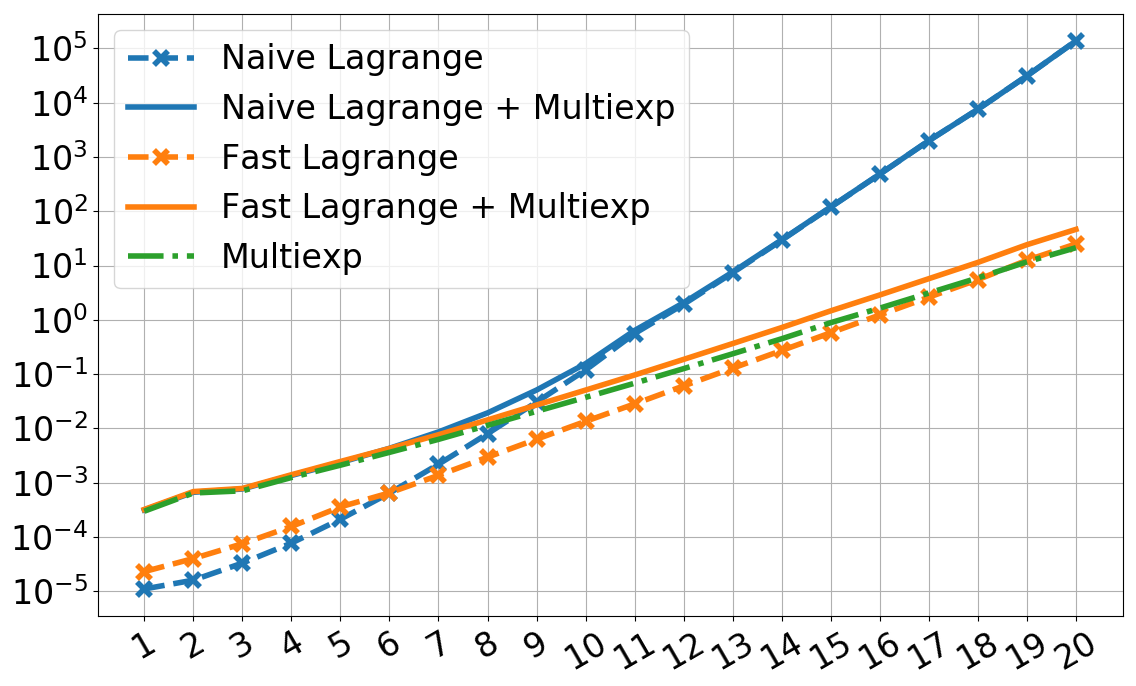
\includegraphics[width=0.70\columnwidth]{figures-thresh/thresh.png}
    \caption{
        This figure plots the time to aggregate a $(t,n)$ BLS TSS (for $t=f+1$ and $n=2f+1$), excluding the share verification cost.
        The $y$ axis is in seconds and the $x$ axis is $\log_2{t}$.
        We plot the individual cost of each aggregation phase: interpolation and multi-exponentiation.
        First, we see that, for BLS with \textit{naive Lagrange}, the signature aggregation cost is dominated by the cost of naive Lagrange interpolation, as $n$ gets larger.
        Second, we see that that our $\Theta(t\log^2{t})$ \textit{fast Lagrange} interpolation beats the $\Theta(t^2)$ naive Lagrange interpolation as early as $t \ge 128$ (or $n \ge 255$).
        Third, as $n$ gets larger, we see that BLS with fast Lagrange is orders of magnitude faster than with naive Lagrange.
    }
    \label{f:thresh}
\end{figure}

First, we sample a random subset of $t$ signers $T$ with valid signature shares $\{\sigma_i\}_{i\in T}$.
Second, we compute Lagrange coefficients $\Ell_i^T(0)$ w.r.t. points $x_i = \omega_N^{i-1}$ (see \cref{s:prelim:interpolation}) using both fast and naive Lagrange.
Third, we compute the final threshold signature $\sigma = \prod_{i\in T} \sigma_i^{\Ell_i^T(0)}$ using a multi-exponentiation.
The measurement configuration for fast Lagrange is $\langle 7 \times 100, 13 \times 10 \rangle$ while for naive Lagrange is $\langle 8\times 100, 6 \times 10, 8, 4, 2, 1,1,1\rangle$.
We plot the average aggregation time in \cref{f:thresh} and observe that our scheme beats the naive scheme as early as $n = \blsOutperformN$.
We do not measure the time to identify valid signature shares via batch verification~\cite{Boldyreva03}, which our techniques leaves unchanged.

Our results show that our fast Lagrange interpolation drastically reduces the time to aggregate when $t\approx n/2$.
Specifically, for $n\approx 2^{21}$, we aggregate a signature in \blsEffTime{2097151}, instead of \blsNaiveTime{2097151} if aggregated via naive Lagrange (\blsTimeImprov{2097151} faster).
The benefits are not as drastic for smaller thresholds, but remain significant.
For example, for $n\approx 2^{15}$, we reduce the time by \blsTimeImprov{32767} from \blsNaiveTime{32767} to \blsEffTime{32767}.
For $n=4095$, we see a \blsTimeImprov{4095} speed-up from \blsNaiveTime{4095} to \blsEffTime{4095}.
For $n=2047$, we see a \blsTimeImprov{2047} speed-up from \blsNaiveTime{2047} to \blsEffTime{2047}.


\subsection{Verifiable Secret Sharing Experiments}
\label{s:eval:vss}
% Note: VSS plots resemble DKG plots
%  VSS deal       ~= DKG per-player deal
%   - but DKG additionally computes f_i(0) proof and NIZKPoK
%  VSS verify     != DKG per-player verify / (n-1)
%   - because DKG also verifies f_i(0) which adds extra work
In this section, we benchmark \evss and \ourvss.
We do not benchmark the complaint round since, when implemented with KZG batch proofs, it remains the same (see \cref{s:scalable-vss:overview}).

\subsubsection{VSS Dealing}
\label{s:eval:vss:deal}

\begin{figure}[t]
    \centering
    \textbf{VSS (and DKG) Dealing Time}\par\medskip
    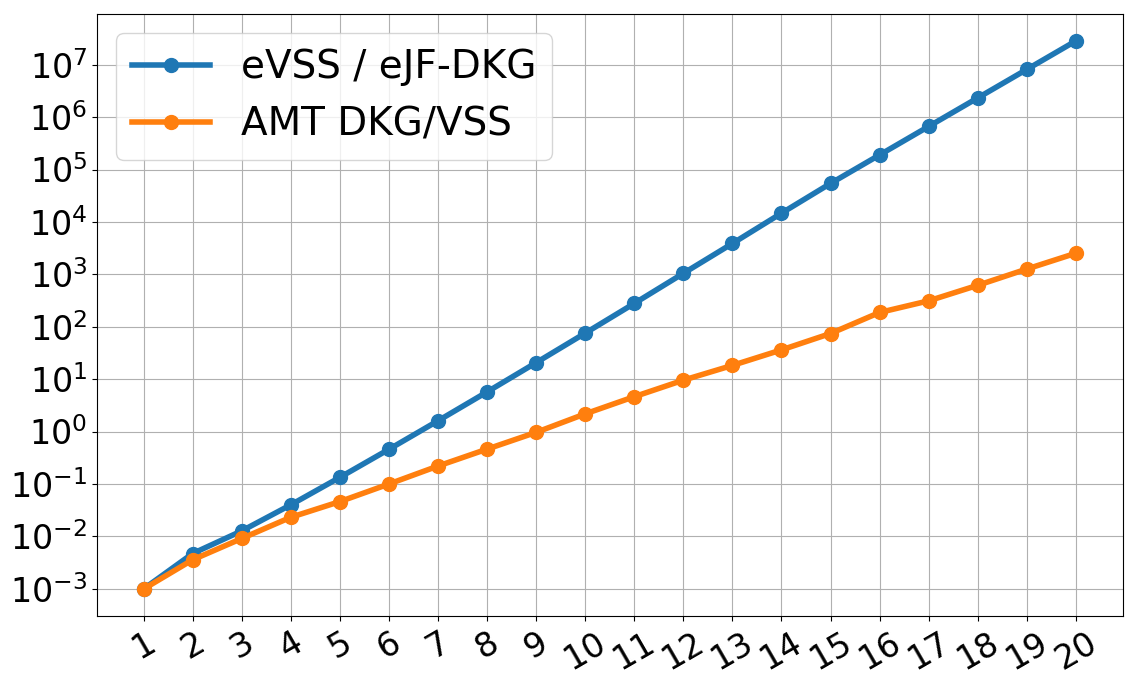
\includegraphics[width=0.70\columnwidth]{figures-thresh/all-deal-times.png}
    \caption{
        This figure shows that our AMT VSS/DKG dealing is orders of magnitude faster than \evss and \ejfdkg dealing. 
        The $y$ axis is the dealing round time in seconds and the $x$ axis is $\log_2{t}$.
        We achieve this speed-up by replacing the $\Theta(tn)$ time KZG proofs with our  $\Theta(n\log{t})$ time AMT proofs.
    }
    \label{f:all-deal-times}
\end{figure}

For \evss dealing, the measurement configuration is $\langle 10 \times 10, 3, 2, 2, 1, 1, 0, 0, 0, 0, 0\rangle$.
For large $t\ge 2^{16}$, \evss dealing is too slow, so we extrapolate it from the previous dealing time (i.e., we multiply by 3.5).
For \ourvss dealing, the measurement configuration is $\langle12 \times 100, 50, 22, 10, 5, 3, 2, 1, 1\rangle$.
In \evss, we compute the shares $s_i$ ``for free'' as remainders of the $\phi(x) / (x-i)$ divisions.
We plot the average dealing time in \ourvss and \evss as a function of $n$ in \cref{f:all-deal-times}.
Our results show that \ourvss's $\Theta(\amtDealTime)$ dealing scales much better than \evss's $\Theta(nt)$ dealing.
For example, for $n\approx 65,000$, \evss takes \evssVssDealTime{65535} while \ourvss takes \amtVssDealTime{65535}.
For very large $n\approx 2^{21}$, \evss takes a prohibitive \evssVssDealTime{2097151} while \ourvss takes \amtVssDealTime{2097151}.
We find that \ourvss's dealing outperforms \evss's as early as $n=\amtVssDealTimeOutperformNevss$.

\subsubsection{VSS Verification Round}
\label{s:eval:vss:share-verif}

\begin{figure}[t]
    \centering
    \textbf{VSS Share Verification Time}\par\medskip
    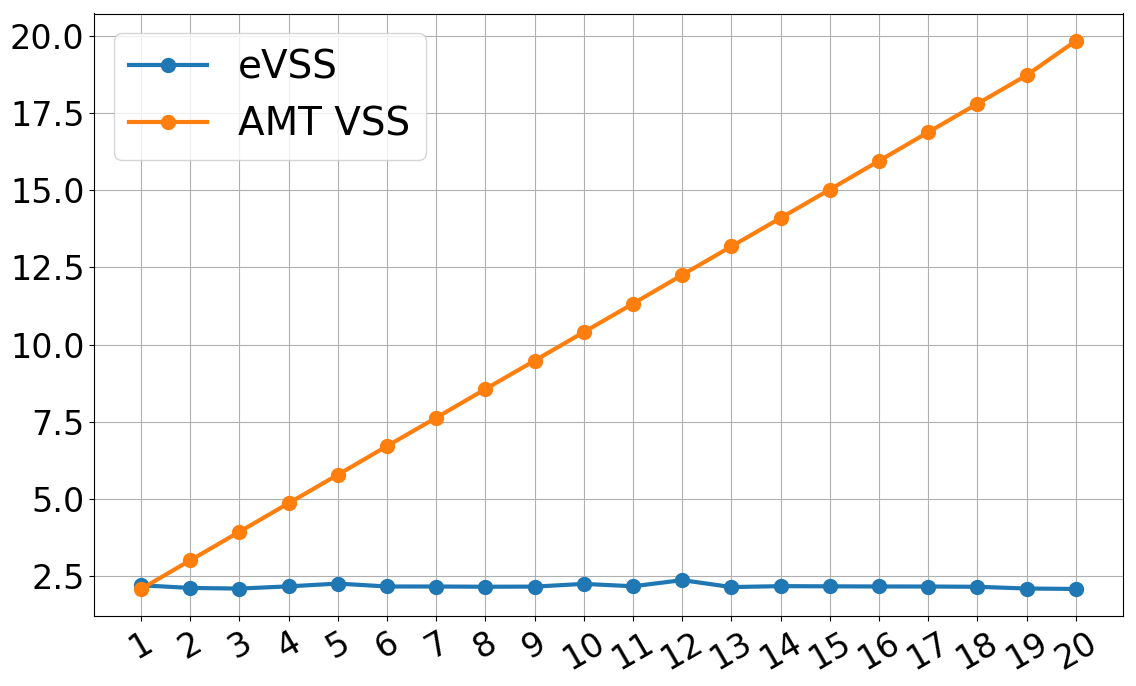
\includegraphics[width=0.70\columnwidth]{figures-thresh/vss-verify-times.png}
    \caption{
        This graph plots the VSS verification round time for both \evss and \ourvss.
        The $y$ axis is the verification round time in milliseconds and the $x$ axis is $\log_2{t}$.
        We can see \ourvss's verification time is slower than \evss (i.e., $\Theta(\amtOneShareVerifTime)$ vs $\Theta(1)$ pairings).
        This is the price we pay for precomputing AMT proofs much faster.
    }
    \label{f:vss-verify-times}
\end{figure}

In \cref{f:vss-verify-times}, we plot the time for one player to verify its share.
The measurement configuration is $\langle 20 \times 1000\rangle$ for both schemes.
In \evss, verification requires two pairings and one exponentiation in $\Group_1$, taking on average $2.15$ ms.
In \ourvss, verification requires $\amtProofSize{t}$ pairings and one exponentiation in $\Group_1$, ranging from \amtVssVerifyTime{3} ($n=3$) to \amtVssVerifyTime{2097151} ($n\approx 2^{21}$).

\subsubsection{VSS Reconstruction}
\label{s:eval:vss:reconstr}

\begin{figure}[t]
    \centering
    \textbf{VSS Reconstruction Time}\par\medskip
    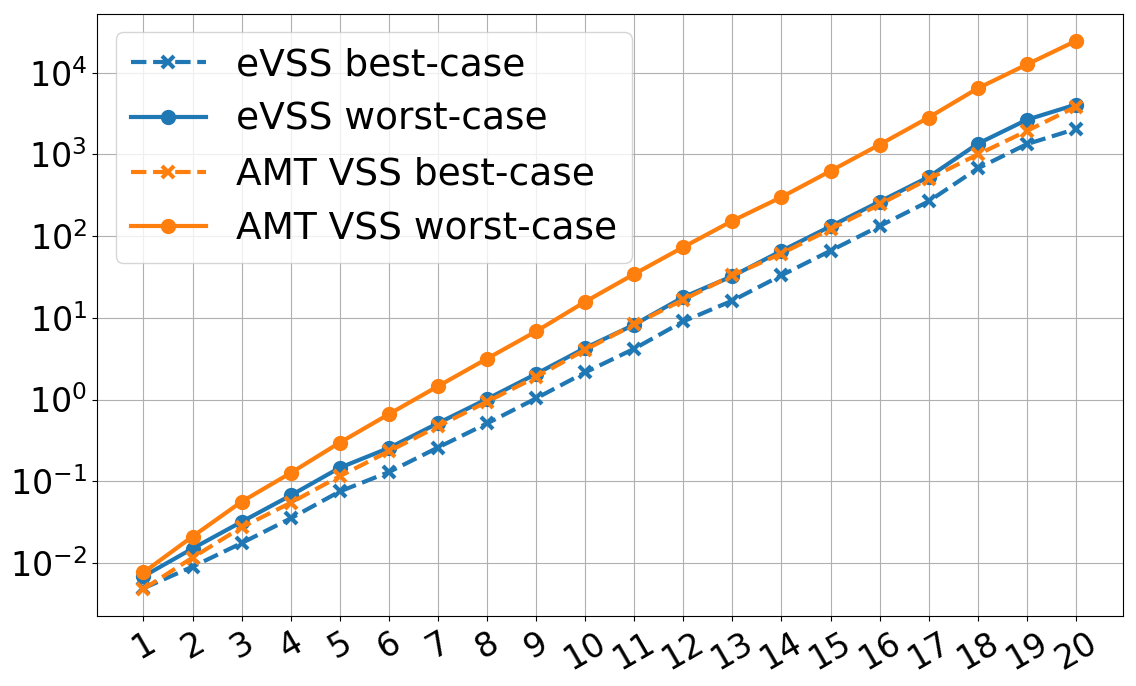
\includegraphics[width=0.70\columnwidth]{figures-thresh/vss-reconstr-times.png}
    \caption{
        This graph shows that \ourvss's reconstruction time is slower than in \evss.
        The $y$ axis is the time in seconds and the $x$ axis is $\log_2{t}$.
        An interesting observation is that \ourvss's best-case reconstruction time is very close to \evss's worst-case reconstruction time (we explain in \cref{s:eval:vss:reconstr} why).
    }
    \label{f:vss-reconstr-times}
\end{figure}

In \cref{f:vss-reconstr-times}, we plot the time to reconstruct the secret.
We consider the \textit{best-case} and \textit{worst-case} times, as detailed in \cref{s:scalable-vss:reconstruction}.
For \evss, ``best case'' means the first $t$ share verifications are successful and ``worst case'' means the first $n-t$ are unsuccessful (see \cref{s:scalable-vss:reconstruction}).
The measurement configuration is $\langle 5 \times 1000, 500, 250, 120, 60, 30, 15, 5\times 10, 8,4,2,1\rangle$ for \evss and $\langle 9 \times 100, 4\times 10, 4,2, 5\times 1\rangle$ for \ourvss.
In both protocols, the (fast) Lagrange interpolation time is insignificant compared to the time to verify shares during reconstruction (e.g., for $n\approx 2^{21}$ in \evss, interpolation is only \fastLagrTime{2097151} out of the total \evssVssReconstrBcTime{2097151} worst-case time).

\ourvss's best-case is very close to \evss's worst-case.
This is because, with the help of memoization, \ourvss's best case only computes $\le 2n-1$ pairings (i.e., the number of nodes in a full binary tree with $n$ leaves).
This closely matches the $2n$ pairings in \evss's worst case.
(In practice, we replace $n$ of these pairings and $\Group_1$ exponentiations by $n$ $\Group_T$ exponentiations, which are slightly faster.)
\ourvss's worst case is \evssVssReconstrWcTimeImprovOveramt{3} to \evssVssReconstrWcTimeImprovOveramt{2097151} slower than \evss's.
But we show next that our faster dealing more than makes up for this.
Finally, \evss's best-case time is half its worst-case time, as expected.

\subsubsection{VSS End-to-End Time}
\label{s:eval:vss:end-to-end}

\begin{figure}[t]
    \centering
    \textbf{VSS End-to-End Time}\par\medskip
    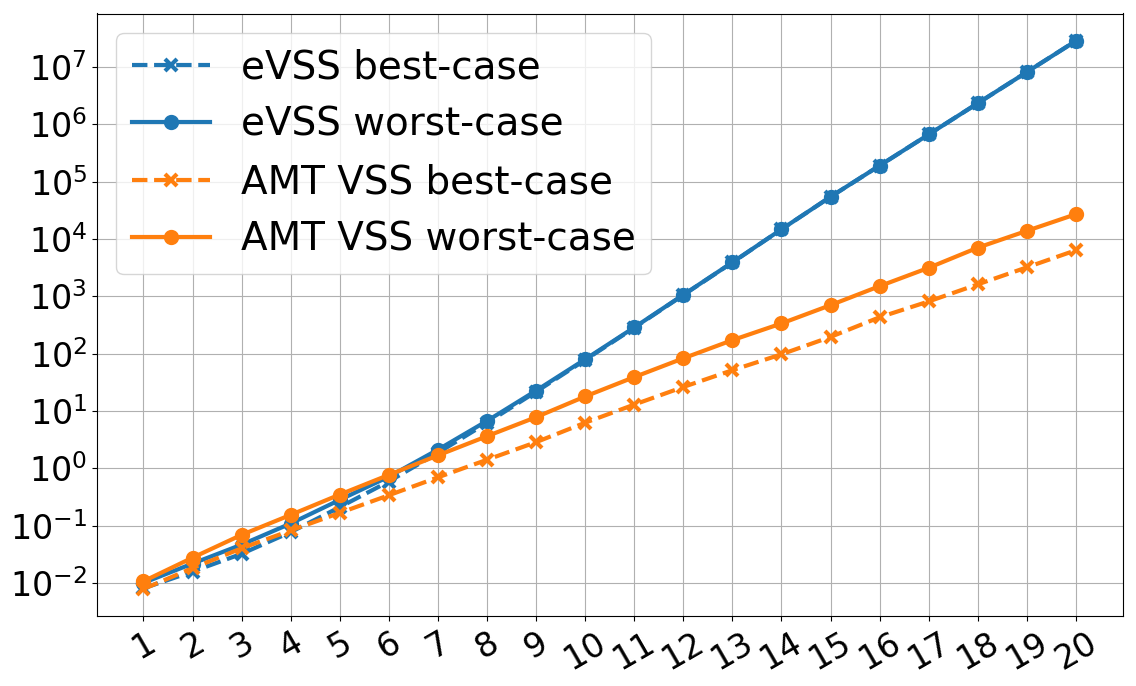
\includegraphics[width=0.70\columnwidth]{figures-thresh/vss-e2e-times.png}
    \caption{
        The $y$ axis is the end-to-end time (i.e., sharing and reconstruction phases) in seconds and the $x$ axis is $\log_2{t}$.
        This graph shows that, in terms of the end-to-end execution time of the VSS protocol, \ourvss is orders of magnitude faster than \evss as $n$ gets larger.
        This is despite our slower verification round and reconstruction phase, which are made up for by our much faster dealing round.
    }
    \label{f:vss-e2e-times}
\end{figure}

Finally, we consider the \textit{end-to-end time}, which is the sum of the sharing and reconstruction phase times.
(Again, a limitation of our work is ignoring the overhead of the complaint round in the worst case.)
\cref{f:vss-e2e-times} gives the best- and worst-case end-to-end times.
The key takeaway is that \ourvss's smaller dealing time makes up for the increase in its verification round and reconstruction phase times.
\ourvss outperforms \evss's worst-case time at $n\ge \vssOutperformWcN$ and its best-case time at $n\ge \vssOutperformBcN$.
For example, for large $n=16,383$, we reduce the worst-case time from \evssVssEndToEndWcTime{16383} to \amtVssEndToEndWcTime{16383} and the best-case time from \evssVssEndToEndBcTime{16383} to \amtVssEndToEndBcTime{16383}.
The best case improvement ranges from \amtVssEndToEndBcTimeImprovOverevss{\vssOutperformBcN} ($n=\vssOutperformBcN$) to \amtVssEndToEndBcTimeImprovOverevss{2097151} ($n\approx 2^{21}$).
The worst case improvement ranges from \amtVssEndToEndWcTimeImprovOverevss{\vssOutperformWcN} ($n=\vssOutperformWcN$) to \amtVssEndToEndWcTimeImprovOverevss{2097151} ($n\approx 2^{21}$).
Thus, we conclude \ourvss scales better than \evss.

\subsection{Distributed Key Generation Experiments}
\label{s:eval:dkg}

Our DKG experiments mostly tell the same story as our VSS experiments:
AMTs drastically reduce the dealing time of DKG players, which more than makes up for the slight increase in verification and reconstruction time.
However, \ourdkg has a \amtDkgCommOverhead{7} to \amtDkgCommOverhead{2097151} communication overhead during dealing.
Still, we believe this is worth the drastic reduction in end-to-end times (see \cref{s:eval:dkg:e2e-time}).

\subsubsection{DKG Dealing}
DKG dealing time is equal to VSS dealing time (see \cref{s:eval:vss:deal}) plus the time to compute a KZG proof and a NIZKPoK for $g^{f_i(0)}$.
However, as $n$ increases, the time to compute these two proofs pales in comparison to the time to compute the $n$ evaluation proofs.
Thus, in \cref{f:all-deal-times}, we treat DKG dealing times as equal to VSS dealing times.
(Having separate VSS and DKG lines in \cref{f:all-deal-times} would be pointless, as they would be almost indistinguishable.)
As a result, the same observations apply here as in \cref{s:eval:vss:deal}: AMTs drastically reduce dealing times.

\subsubsection{DKG Verification Round}
\label{s:eval:dkg:share-verif}

\begin{figure}[t]
    \centering
    \textbf{DKG Share Verification Round Time}\par\medskip
    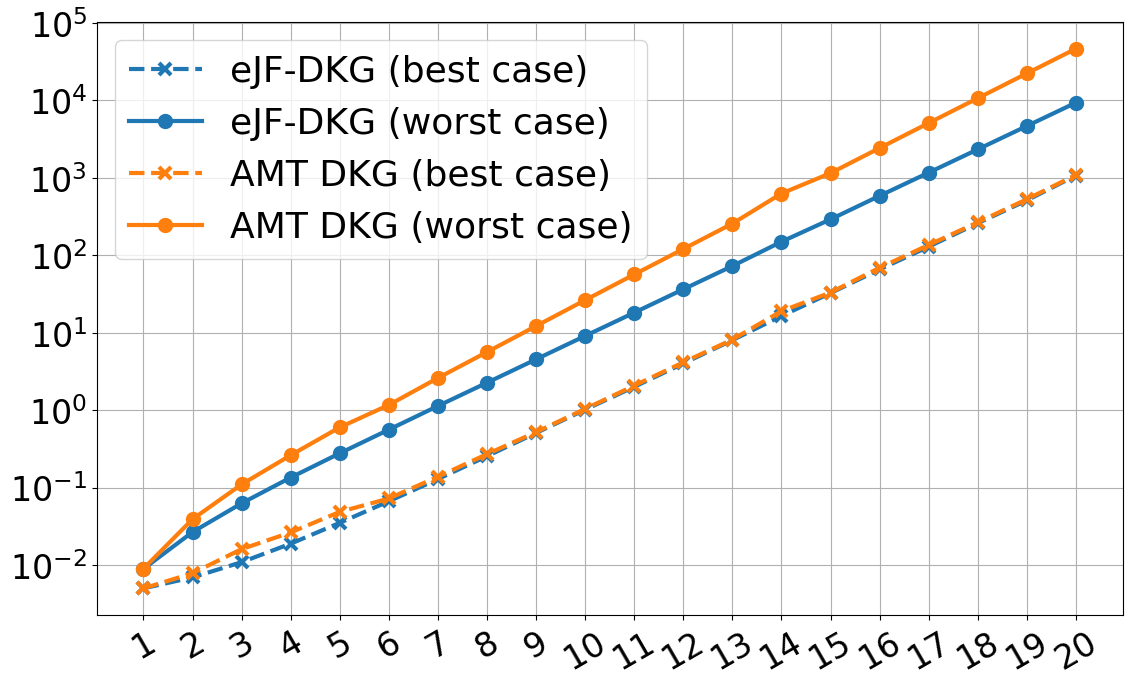
\includegraphics[width=0.70\columnwidth]{figures-thresh/dkg-verify-times.png}
    \caption{
        The $y$ axis is the verification round time in seconds and the $x$ axis is $\log_2{t}$.
        This graph shows that \ourdkg's \textit{worst-case} share verification round is slower than \ejfdkg's.
        This is due to our $\Theta(\amtAllShareVerifTime)$ cost to verify all $n$ shares, compared to \ejfdkg's $\Theta(n)$ cost.
        However, in the \textit{best case}, both protocols perform almost the same, since most of the time is spent aggregating proofs instead of verifying them.
    }
    \label{f:dkg-verify-times}
\end{figure}

We consider both the \textit{best case} and the \textit{worst case} verification time, as discussed in \cref{s:scalable-dkg:share-verif}.
In our best-case experiment, each player $j$ aggregates all its shares as $s_j=\sum_{i\in[n]} s_{i,j}$ and their evaluation proofs as $\pi_j$.
Then, $j$ verifies $s_j$ against $\pi_j$.
Similarly, $j$ aggregates and efficiently verifies all its $g^{f_i(0)}$'s and their KZG proofs.
In the worst-case experiment, $j$ individually verifies the $s_{i,j}$ shares and the $g^{f_i(0)}$'s.
Importantly, in both experiments, $j$ individually verifies all $n$ NIZKPoKs for $g^{f_i(0)}$ in $\Theta(n)$ time.
The two experiments are meant to bound the time of a realistic implementation that carefully uses \textit{batch verification}~\cite{Boldyreva03,LM07} to not exceed the worst-case time too much.

The best-case \ejfdkg measurement configuration is $\langle 8 \times 100, 50, 25, 12, 9 \times 10\rangle$ and the worst-case is $\langle 5 \times 100, 50, 25, 12, 12\times 10 \rangle$.
For \ourdkg, the best-case configuration is $\langle 12\times 100, 80, 40, 20, 16, 8, 4, 3, 2 \rangle$ and the worst-case is $\langle 5 \times 100, 4\times 80, 40, 20, 8, 4, 2, 6\times 1 \rangle$.
The average per-player verification times are plotted in \cref{f:dkg-verify-times}.
In the best case, both schemes perform roughly the same, since the verification of the $n$ NIZKPoKs quickly starts dominating the aggregated proof verification.
In the worst case, \ourdkg time ranges from \amtDkgVerifyWcTime{3} ($n=3$) to \amtDkgVerifyWcTime{2097151} ($n \approx 2^{21}$).
In contrast, \ejfdkg time ranges from \ejfDkgVerifyWcTime{3} to \ejfDkgVerifyWcTime{2097151} (\ejfDkgVerifyWcTimeImprovOveramt{7} to \ejfDkgVerifyWcTimeImprovOveramt{2097151} faster).
Nonetheless, \ejfdkg remains slower overall due to its much slower dealing (see \cref{s:eval:dkg:e2e-time}).
Both best- and worst-case times can be reduced by batch-verifying NIZKPoKs, which resemble Schnorr signatures~\cite{Schnorr89} and are amenable to batching~\cite{BDL+12}.

\subsubsection{DKG Reconstruction}
\label{s:eval:dkg:reconstr}

\begin{figure}[t]
    \centering
    \textbf{DKG Reconstruction Time}\par\medskip
    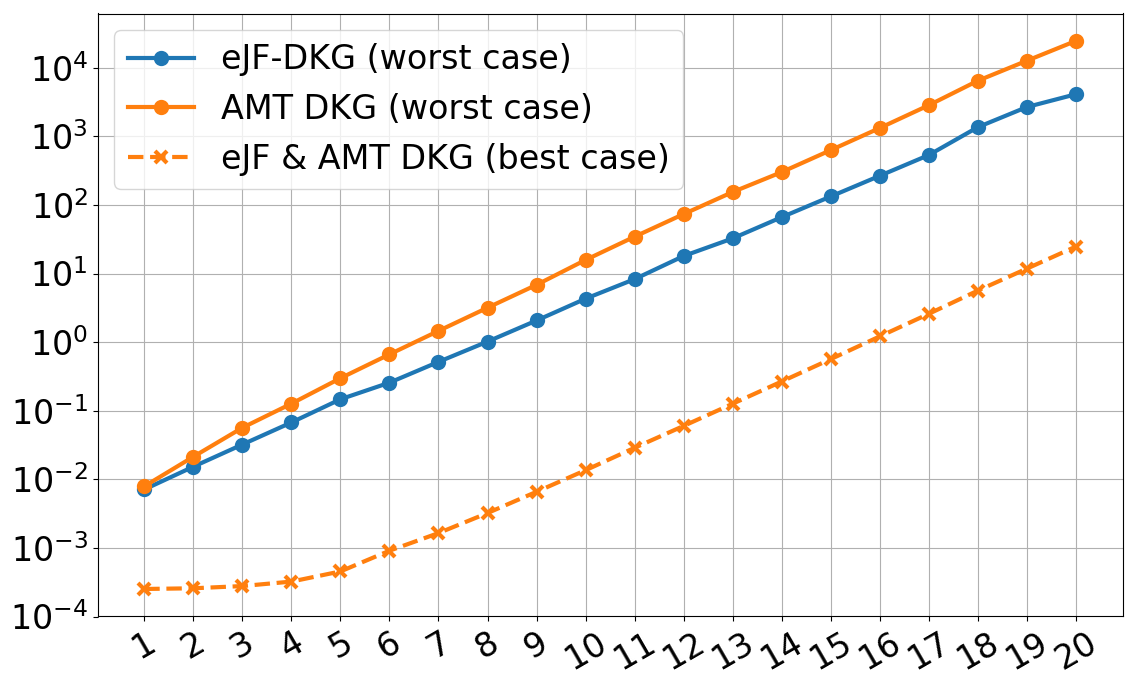
\includegraphics[width=0.70\columnwidth]{figures-thresh/dkg-reconstr-times.png}
    \caption{
        The $y$ axis is the reconstruction phase time in seconds and the $x$ axis is $\log_2{t}$.
        This graph shows that, in the \textit{best case}, both \ourdkg and \ejfdkg are just as fast, since they both just interpolate the secret $s$ directly.
        In the \textit{worst case}, however, \ourdkg has to spend more time verifying shares than \ejfdkg due to our larger proofs.
        Nonetheless, in \cref{f:dkg-e2e-times}, we show our slower reconstruction time is worth it, since our end-to-end time is much smaller than in \ejfdkg.
    }
    \label{f:dkg-reconstr-times}
\end{figure}

Here the measurement configuration is $\langle 4\times 1000, 200, 50, 25, 13\times 10\rangle$ and times are plotted in \cref{f:dkg-reconstr-times}.
The best case is very fast in both \ejfdkg and \ourdkg, taking only \amtDkgReconstrBcTime{2097151} for $t=2^{20}$, since both schemes interpolate the secret $s$ without verifying shares and check it against $g^s$ (see \cref{s:scalable-dkg:reconstr}).
For the worst case, the time is the sum of (1) the (failed) best-case reconstruction time and (2) the worst-case time to identify $t$ valid shares from $n$ shares.
Since the best case is very fast, the DKG worst-case time (see \cref{f:dkg-reconstr-times}) looks almost identical to its VSS counterpart (see \cref{f:vss-reconstr-times}).
Note that the same \ourvss speed-up techniques for finding $t$ valid shares apply in \ourdkg (see \cref{s:scalable-vss:reconstruction}).
\ourdkg's worst case is anywhere from \ejfDkgReconstrWcTimeImprovOveramt{3} to \ejfDkgReconstrWcTimeImprovOveramt{2097151} slower than \ejfdkg's, much like \ourvss.
However, as we show next, \ourdkg's faster dealing more than makes up for this.

\subsubsection{DKG End-to-End Time}
\label{s:eval:dkg:e2e-time}

\begin{figure}[t]
    \centering
    \textbf{DKG End-to-End Time}\par\medskip
    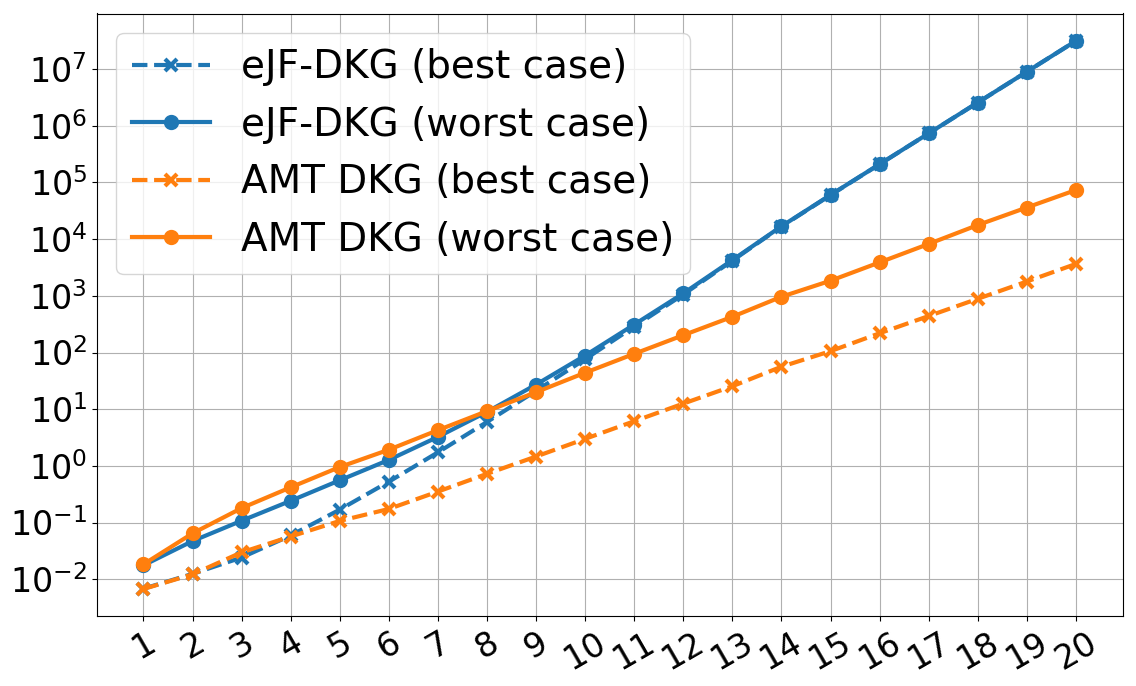
\includegraphics[width=0.70\columnwidth]{figures-thresh/dkg-e2e-times.png}
    \caption{
        The $y$ axis is the end-to-end time (i.e., sharing and reconstruction phases) in seconds and the $x$ axis is $\log_2{t}$.
        This graph shows that, in terms of the end-to-end execution time of the DKG protocol, \ourdkg is orders of magnitude faster than \ejfdkg as $n$ gets larger.
        This is because our slower verification round and reconstruction phase are more than made up for by our much faster dealing round.
    }
    \label{f:dkg-e2e-times}
\end{figure}

Similar to the VSS experiments in \cref{s:eval:vss:end-to-end}, we consider the \textit{end-to-end time}.
\cref{f:dkg-e2e-times} plots the best- and worst-case end-to-end times and shows that \ourdkg outperforms \ejfdkg starting at $n\ge \dkgOutperformBcN$ (in the best case) and at $n\ge\dkgOutperformWcN$ (in the worst case).
This is a direct consequence of \ourvss outperforming \evss, since the DKG protocols use these VSS protocols internally.
For example, for large $n=16,383$, we reduce the worst-case end-to-end time from \ejfDkgEndToEndWcTime{16383} to \amtDkgEndToEndWcTime{16383} and the best-case time from \ejfDkgEndToEndBcTime{16383} to \amtDkgEndToEndBcTime{16383}.
The improvement in best-case end-to-end time ranges from \amtDkgEndToEndBcTimeImprovOverejf{\dkgOutperformBcN} ($n=\dkgOutperformBcN$) to \amtDkgEndToEndBcTimeImprovOverejf{2097151} $(n\approx2^{21})$ and, in the worst case, from \amtDkgEndToEndWcTimeImprovOverejf{\dkgOutperformWcN} to \amtDkgEndToEndWcTimeImprovOverejf{2097151}.
Thus, we conclude \ourdkg scales better than \ejfdkg.

\subsubsection{DKG Communication}
\label{s:eval:dkg:communication}

\begin{figure}[t]
    \centering
    \textbf{DKG Communication}\par\medskip
    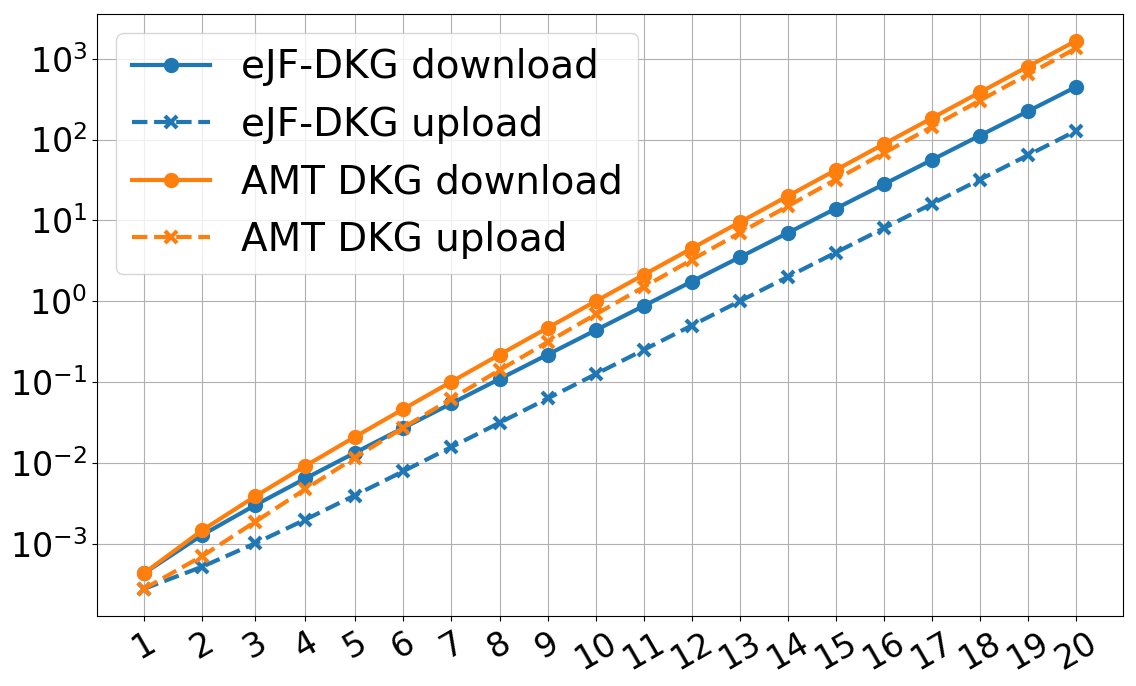
\includegraphics[width=0.70\columnwidth]{figures-thresh/bw.png}
    \caption{
        The $y$ axis is the communication in mebibytes (MiBs) and the $x$ axis is $\log_2{t}$.
        This graph shows that \ourdkg incurs slightly higher communication than \ejfdkg.
        % Note: For some reason, my more complicated macros don't work inside \caption without \protect.
        The per-player upload during dealing increases by at most \protect \amtDkgUploadOverhead{2097151} and the download by at most \protect \amtDkgDownloadOverhead{2097151}.
        Overall, \ourdkg's communication overhead ranges from \protect \amtDkgCommOverhead{3} to \protect \amtDkgCommOverhead{2097151}.
    }
    \label{f:dkg-bw}
\end{figure}

We estimate each player's upload and download during the dealing round.
For upload, each \ejfdkg and \ourdkg player $i$ has to broadcast a KZG commitment $g^{f_i(\tau)}$ (32 bytes) and a commitment $g^{f_i(0)}$ with a NIZKPoK and a KZG proof (32 + 64 + 32 bytes).
Then, $i$ has to send each $j\in[n]$ its share (32 bytes) with an evaluation proof (32 bytes for KZG or $(\amtProofSize{t}) \cdot 32$ bytes for AMT).
For download, each player $i$, has to download $n-1$ shares, each with their KZG commitment and evaluation proof, plus $n-1$ $g^{f_j(0)}$'s, each with their NIZKPoK and KZG proof.
Note that \ourdkg uses KZG proofs for $g^{f_i(0)}$ to minimize its communication overhead.

We plot the upload and download numbers for both schemes in \cref{f:dkg-bw}.
\ejfdkg's per-player upload ranges from \ejfDkgUpload{3} to \ejfDkgUpload{2097151} while download ranges from \ejfDkgDownload{3} to \ejfDkgDownload{2097151}.
\ourvss's upload overhead ranges from \amtDkgUploadOverhead{3} to \amtDkgUploadOverhead{2097151} and its download overhead ranges from \amtDkgDownloadOverhead{3} to \amtDkgDownloadOverhead{2097151}.
Overall, \ourvss's upload-and-download overhead ranges from \amtDkgCommOverhead{3} to \amtDkgCommOverhead{2097151}.
Thus, we believe the \amtDkgEndToEndBcTimeImprovOverejf{2097151} and \amtDkgEndToEndWcTimeImprovOverejf{2097151} reductions in best- and worst-case end-to-end times are sufficiently large to make up for this overhead.